\documentclass[10pt, a4paper]{article}
\usepackage{lrec}
%\usepackage{multibib}
%\newcites{languageresource}{Language Resources}
\usepackage{graphicx}
\usepackage{tabularx}
\usepackage{soul}
% for eps graphics

\usepackage{epstopdf}
\usepackage[latin1]{inputenc}

\usepackage{hyperref}
\usepackage{xstring}

\newcommand{\secref}[1]{\StrSubstitute{\getrefnumber{#1}}{.}{ }}

\title{Annotating Abstract Meaning Representations for Spanish}

\name{Noelia Migueles-Abraira, Rodrigo Agerri, Arantza Diaz de Ilarraza}

\address{IXA NLP Group, University of the Basque Country UPV/EHU\\
         noeliamigueles@gmail.com,\{rodrigo.agerri,a.diazdeilarraza\}@ehu.eus}


\abstract{
Until recently, semantic annotations for different semantic phenomena were independent and unconnected. The Abstract Meaning Representation (AMR) project arised out of the need to create a broad-coverage semantic bank containing a unified set of semantic information represented in simple, single-rooted, easy-to-read structures. Because the semantic representation language proposed in AMR is biased towards English, annotating AMR structures for other languages, such as Spanish, is not a trivial task. In this paper we propose a linguistic method that we believe would help lay the groundwork for building a large semantic bank for Spanish and would guide those who would like to implement it for other languages. Thus, we analyze a broad spectrum of Spanish linguistic phenomena to come up with suggestions to adapt the current guidelines so that it is possible to annotate AMRs for Spanish. As a result of this work, we make available the first public online repository containing manually annotated Spanish AMRs.\\ \newline \Keywords{AMR, Sembank, Semantics, Spanish Language Resources} }

\begin{document}

\maketitleabstract

\section{Introduction}

The construction of large manually annotated corpora has been crucial in order to advance Natural Language Processing (NLP) technology. Among others, the construction of the Penn Treebank \cite{marcus_building_1993} made possible the existence of many statistical parsers trained on syntactic treebanks which perform at an accuracy of about 90\% \cite{charniak_coarse--fine_2005}. In contrast, computational semantics is lagging behind in this respect, as most of the semantic annotated resources for English are rather scattered or simply nonexistent for the large majority of languages.

This lack of a unified sembank of natural language sentences paired with their sentential, logical meanings is what led to the appearance of Abstract Meaning Representation (AMR), a semantic representation language introduced by \cite{banarescu2013abstract}. This approach promotes the representation of the logical meaning of sentences as single rooted, directed graphs (or AMRs) with labelled nodes (concepts) and edges between them (relations). These incorporate semantic roles, among other linguistic phenomena. In a propositional-style logic, AMR is able to capture who is doing what to whom in a sentence. Furthermore, AMR tries to abstract away from both morphological and syntactic idiosyncrasies that account for several cross-lingual differences. However, there is still a problem with this approach, as it is strongly biased (by design) to annotate English sentences. To overcome this fundamental limitation, we decided to explore the possibility of annotating AMRs for Spanish texts.

Thus, the central goal of this work is to investigate how to create Spanish AMRs in order to build a sizable Spanish sembank. We address this objective by answering the following questions:

\begin{enumerate}
\item Is it possible to follow the current guidelines to annotate Spanish AMRs? And if not, how can the guidelines be refined in order to annotate Spanish AMRs? Also, what resources do we need to carry out such task?
\item How similar are English and Spanish AMRs?
\item What can be learned from the gathered information for future annotation efforts?
\end{enumerate}

The result of this study has made it possible to manually annotate, for the first time, a Spanish corpus with AMR structures. Furthermore, we believe that our study will help laying the groundwork for building a large semantic bank for Spanish as well as a reference for other languages.

\begin{figure}[!h]
\begin{center}
%\fbox{\parbox{6cm}{
%This is a figure with a caption.}}
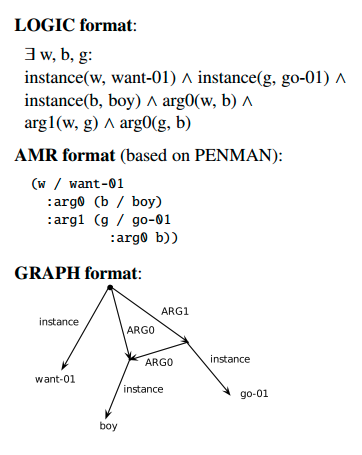
\includegraphics[scale=0.5]{banarescu-amr-example}
\caption{Equivalent formats for representating the meaning of
``The boy wants to go'' according to Banarescu et al. (2013).}
\label{fig:amr-example}
\end{center}
\end{figure}
Prior to this study, other had worked on the adaptation of AMR to different languages besides English (\cite{uresovaetal14}; \cite{lietal16};  \cite{xueetal14}) . For the moment, however, only a small bank of non-English sentences paired with their semantic representations is available to the public\footnote{The Chinese Abstract Meaning Representation (CAMR) Bank is available at:\url{http://www.cs.brandeis.edu/~clp/camr/camr.html}}.

\section{Background}\label{sec:background}

AMR as a semantic representation language appears based on the assumption that we lack a simple readable semantic bank of natural language sentences ``paired with their whole-sentence, logical meanings'' \cite{banarescu2013abstract}. Thus, they started annotating the logical meaning of sentences, for which a particular sentence is encoded as a Directed Acyclic Graph (DAG). The ultimate goal is to encourage advances in different NLP tasks, including Statistical Natural Language Understanding (SNLU) or Statistical Machine Translation (SMT), amongst others. The idea is to do this by enabling rapid human annotation of broad coverage corpora. Some phenomena that AMR addresses include discourse connectives, semantic roles, intrasentential coreference, named entities (and wikification), questions, negation, and modality. AMR features a three-way annotation format: a logic-based format \cite{Davidson:1980}, an AMR format, and a graph format. The three are equivalent. An example can be seen in Figure \ref{fig:amr-example}.

AMR strives to capture many aspects of meaning in a single simple data structure. To do that, it tries to abstract away from morpho-syntactic idiosyncrasies. AMR uses PropBank (PB) framesets \cite{kingsbury_treebank_2002}. Thus, each frame presents annotators with a list of senses which contains its own number of core arguments. AMR defines around a hundred semantic relations. These relations consist of core ``:ARGX'' roles (frame arguments), non-core roles (general semantic relations), roles for quantities, for date-entities, operators such as ``:opX'' and ``:prep-X'', multi-sentence roles, and a conjunction role. Simple roles often correspond to a reified concept. AMR does not dictate a mandatory way of applying rules. Instead, it promotes personal interpretation of researchers about how strings are related to meanings. For specific details about AMR annotation guidelines, please read Banarescu et al. (2013)\footnote{Also, the more detailed annotation guidelines are available here: \url{https://github.com/amrisi/amr-guidelines/blob/master/amr.md}}.

\section{Methodology}\label{sec:methodology}

Our methodology aims to determine whether if it is possible to annotate Spanish meaning representations following the current Abstract Meaning Representation (AMR) guidelines. The key is to detect aspects of meaning in Spanish sentences that cannot be represented when applying the current AMR guidelines. After the identification of such relevant linguistic aspects, we propose a new set of guidelines so that the annotation of these within the AMR framework will be possible. During the preliminary stage of this phase, we manually created a sample of Spanish AMRs according to the original AMR annotation scheme. Next, we identified any missing aspects of meaning that AMR failed to represent. Finally, we designed an extension of the annotation scheme to potentially meet those needs. This refinement in the AMR annotation standard stays true to the AMR syntax.

To carry out this analysis, we decided to use The Little Prince Corpus\footnote{\url{https://amr.isi.edu/download.html}}. The corpus contains 1652 sentences represented in AMR structures for both English and Chinese. As the AMR project points out, using this freely available corpus would allow researchers to compare different representations of the same text. The selection of these sentences was not a random process. First, we translated about 250 sentences from The Little Prince. Then, we made a comparison between the resulting pairs of English-Spanish sentences. Out of those, we narrowed down the number to 50, resulting in a selection of sentences that includes a wide range of linguistic phenomena, including nominal ellipses, clitic pronouns, gender, verbal periphrases and locutions, double negatives, nominalization and verbalization, affixes, and some key words that have a special treatment in AMR. To choose these, we also paid attention to the level of structural cross-lingual variation that the sentence pairs exhibit, just so we could study both language pairs whose structures align well and those whose structures do not align well. Declarative, interrogative, exclamatory, and imperative sentences are covered. For our purpose, we consider that this number of sentences, in spite of being small, is good enough to detect a reasonable amount of Spanish-specific constructions that the current English-only version of AMR is not able to represent.

The following section details the main Spanish linguistic phenomena identified in this study and the solutions we propose in order to provide an AMR representation addressing them.

\section{Annotation Examples}\label{sec:annotation-examples}

We have identified seven main Spanish linguistic phenomena that cannot be represented in AMR under the current guidelines: NP ellipses, third person possessive pronouns, third person clitic pronouns, the usage of \textit{se}, gender, certain verbal constructions such as verbal periphrases and locutions, and double negatives. We therefore decide to extend the AMR annotation guidelines to be able to annotate such cases \cite{migueles2017study}. For space reasons, in this paper we discuss the first 4 out of these 7 phenomena. Before we start, though, it is important to explain why we chose to adapt the current guidelines by converting some roles, reifications, modals, and special words into their Spanish counterparts. This need arises from the fact that sometimes certain roles and relations which receive a special treatment in AMR lead to confusion if we try to use them as such in Spanish. For instance, many roles like ``:prep-X'' present a problem. Not only because the annotator may not know to which such role is referring to but also because the equivalences between Spanish and English prepositions might not be straightforward, one-to-one correspondences. For example, the English equivalents for the Spanish preposition \emph{en} could be one of the following: ``in'', ``inside'', ``into'', ``within'', or ``by''. In such case, an annotator would have to figure out which preposition should be used, and how, because not all prepositions are annotated with the role ``:prep-X.''. To solve this and other issues, we propose the conversion of roles, reifications, modals, and special words from English to Spanish. Hence, from now onwards, we will apply such conversions (see \cite{migueles2017study} for more details).

\subsection{NP Ellipses}

Because of the nature of Spanish grammar, nominal ellipsis in Spanish is pervasive. In most cases, we will find either a conjugated verb and/or a clitic pronoun that indicates person. So, technically, there is no need to add a Noun Phrase (NP) unless we need to clarify the subject.

\begin{enumerate}
\item[(1)]Carla tiene prisa. Tiene cita con el dentista.\\
Carla is in a hurry. (She) has an appointment with the dentist.
\end{enumerate}

If we look at the second sentence on its own, we know that we are talking about a single female entity in the English version. In Spanish, however, we do not. While annotating the English version, one would add "she" rather than "he" or "it" as the entity that has an appointment with the dentist. Unfortunately, in the Spanish version, the only information that we have about such entity is that it refers to a second-person singular entity. There is a reference to an entity, even if we do not know which entity due to a lack of content (remember that AMR treats the semantic meaning of single sentences). The same would happen with the plural pronoun "they" - as it would be addressed in the sentence. However, the Spanish version \textit{Tienen cita con el dentista} could imply that the entity is either the plural form \emph{ellos} (masculine or generic masculine) or the plural form \emph{ellas} (feminine). The ellipsis in this case has left the gender of the agent role underspecified. If we represent such sentence following AMR guidelines, we do not explicitly state that there is such underspecification. 

\begin{verbatim}
(t / tener
    :ARG1 (c/cita
    :prep-con (d / dentista)))
\end{verbatim}

Thus, whenever there is a nominal ellipsis, we propose to use a concept \emph{ente} (``being'') that is mapped to a non-core role \emph{:sinnombre} (``:nameless'') and followed by a concept of the same name. This decision is based on the idea that not including an entity that performs an action in the annotation, when the sentence evidently states that there is one, would lead to an inaccurate semantic meaning representation. If there is a referenced -- or, at least, partially referenced -- entity, the logical thing to do would be to add such entity to the resulting AMR. Below there is an example of the proposed annotation of a third person nominal ellipsis following this new rule.

\begin{verbatim}
(t / tener
    :ARG0 (e / ente
        :sinnombre (s / sinnombre))
    :ARG1 (c / cita
        :prep-con (d / dentista)))
\end{verbatim}

As we can see in this example, the concept \textit{ente} would be related to the root node \textit{tener}. In the English AMR, this would actually correspond to the concept "she."

\begin{verbatim}
(h / have-03
    :ARG0 (s / she)
    :ARG1 (a / appointment-02
        :ARG0 s
        :ARG1 (d/ dentist)))
\end{verbatim}

\subsection{Third Person Possessive Pronouns}\label{sec:third-pers-poss}

When it comes to annotate ellipses in possessive NPs, another issue arises. This has to do with the third person singular and plural possessive pronouns \emph{su} and \emph{sus}. The problem, once again, is not knowing much about the possessor. For instance, \emph{su} could be translated as ``his'', ``her'', ``its'', ``they,'' or even ``your'' (formal language). The difference here -- unlike in the previous phenomenon -- is that the possessive entity is actually present in the sentence. AMR currently marks possession using a \emph{:posee} operator following by the concept (his, her, its, etc.). Given that for Spanish this is underspecified, the argument of the operator \emph{:posee} should be \emph{su} but we need to explicitly state that its meaning is not fully specified. Again, bear in mind that to know the exact entity to which any of these pronouns is referring to, one needs to have access to contextual information. Because AMR only looks at individual sentences, we are not sure who the possessor is. Then, rather than implying that the possessor is "he", "she", "they," or "you" without really knowing if that is the case, whenever there is ellipsis in possessive NPs, we also annotate an entity with the concept \emph{ente}. This, however, is tagged with the non-core role \emph{:sinespecificar} (``:unspecified''). The latter is followed by the possessive pronoun in singular form, as it is shown in the following AMR structure:

\begin{enumerate}
\item[(2)]Su casa es grande.\\
(His/her/its/your) house is big.
\end{enumerate}

\begin{verbatim}
(g / grande
    :campo (c / casa
        :posee (e / ente
            :sinespecificar (s / su))))
\end{verbatim}


\begin{figure*}[ht]
\begin{center}
%\fbox{\parbox{6cm}{
%This is a figure with a caption.}}
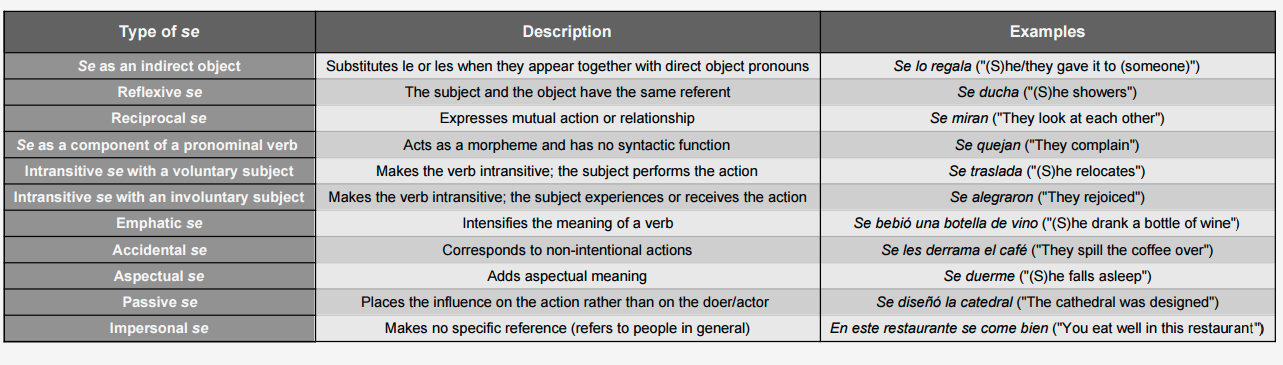
\includegraphics[scale=0.35]{se-usage}
\caption{\emph{Se} usage with examples according to Lozano (2005)}
\label{fig:se-usage}
\end{center}
\end{figure*}

\subsection{Third Person Clitic Pronouns}\label{sec:third-person-clitic}

A similar complication occurs when attempting to annotate third person clitic pronouns. Consider the following example in which \emph{lo}, as a clitic pronoun, fails to provide much information of the entity that it refers to because it is semantically underspecified. As far as we know, it could be equally associated to an animate or inanimate being. For instance, we could break down the word \emph{m\'andaselo} into three components: \emph{manda} $+$ \emph{se} $+$ \emph{lo}, where  \emph{manda} is the second person singular of the verb \emph{mandar} (``to send''), \emph{se} is an enclitic pronoun that means ``to (him/her/it)'' and \emph{lo} is another enclitic pronoun that refers to an underspecified entity in third person singular. 

\begin{enumerate}
\item[(3)]M\'andaselo ahora.\\
Sent (it/him) to (him/her/it) now.
\end{enumerate}

Once again, following the idea that ignoring a present entity would lead to an inaccurate semantic meaning representation, we generally annotate enclitic and proclitic pronouns in the same way that we annotate third-person possessive NPs to cover this information. Consider the next annotation.
\begin{verbatim}
(m / mandar
    :modo imperativo
    :ARG0 (t / tu)
    :ARG1 (e / ente
        :sinespecificar (l / lo))
    :ARG2 (e2 / ente
        :sinespecificar (s / se))
    :tiempo (a / ahora))
\end{verbatim}

Constructions of this kind tend to be quite straightforward in English (see example below). But in Spanish, the semantic meaning may not be that clear without taking previous sentences into consideration. To not come up with either an incorrect or too ambiguous annotation, we consider the use of this relation to help the system. For instance, while translating AMRs to plain text.

\begin{verbatim}
(s / send-01
    :ARG0 (y / you)
    :ARG1 (i / it)
    :ARG2 (h / he)
    :time (n / now))
\end{verbatim}

\subsection{\emph{Se} Usage}
{
With at least eleven uses (Figure \ref{fig:se-usage}), \emph{se} is quite possibly the most versatile pronoun in the Spanish language (\cite{lozanose};\cite{millanusose}; \cite{haywood2008thinking}). In most cases, the problem that we encounter is not knowing who or what is the direct or the indirect object. As seen in the previous example \emph{m\'andaselo ahora}, we simply do not know to whom (or what) it needs to be sent. Only context could tell us that but AMR currently does not focus on the analysis of interconnected sentences. At this point, we are left with no other choice but to include something to cover semantic underspecification. To do that, we follow the aforementioned clitic  annotation procedure. Semantic underspecification is also the norm for the rest of the uses of \emph{se}. However, the solutions provided to represent each use in AMR vary. Thus, when \emph{se} is reflexive, we use reentrancy, as we can see in the AMRs below:

\begin{enumerate}
\item[(4)]Se gusta.\\
(She/he/it) likes (her/him/it)self.
\end{enumerate}

\begin{verbatim}
(g / gustar
    :ARG0 (e  / ente
        :sinespecificar (s / se))
    :ARG1 e)
\end{verbatim}

The criterion to annotate reciprocal \emph{se} is slightly different. We also use reentrancy, but we add a concept named \emph{se-rec\'iproco} (\emph{reciprocal-se}).

\begin{enumerate}
\item[(5)]Se gustan.\\
They like each other.
\end{enumerate}

\begin{verbatim}
Se gustan.
(g / gustar
    :ARG0 (e / ente
        :sinespecificar (s / se-reciproco))
    :ARG1 e)
\end{verbatim}

Note the difference with the English equivalent:

\begin{verbatim}
(l / like-01
    :ARG1 (e / each
        :mod (o / other)))
\end{verbatim}

If we consider impersonal and passive usages of \emph{se}, a different issue applies. Once again, we do not know who or what performs a given action. However, in these cases there is no subject that is explicitly stated in the sentence.

\begin{enumerate}
\item[(6)]Se vende casa rural.\\
Country house on sale.
\end{enumerate}

\begin{verbatim}
(v / vender
    :ARG1 (c / casa
    :mod (r / rural)))
\end{verbatim}

% \section{Related Work}\label{sec:related-work}

% Recent studies for adapting it to other languages (Uresova et al., 2014; Li et al. 2016) have been done. But at the moment, there is only a small, publicly available corpus in a language other than English (REF)

\section{Concluding Remarks}

This research project is the first step towards the construction of a sizable sembank of Spanish sentences paired with their sentential, logical meanings. Our main goal was to study how to create Spanish Abstract Meaning Representations (AMRs).

As we have seen, the current guidelines, as they are, fail to represent Spanish semantic representations fully. This is no surprise, since it is clearly stated in the guidelines that AMR is not an interlingua. On a positive note, we have demonstrated that it is, in fact, possible to adjust the guidelines accordingly to cover their lack of certain meaning aspects in Spanish that cannot be ignored. To annotate Spanish AMRs, we need the guidelines to be adapted for this task, and we need an editor that is connected to a refined and updated version of AncoraNet \cite{taule2008ancora}.

Although a substantial amount of work remains to be done, the information that we have 	obtained serves as the foundation for future work. Because of this study, we now know what is needed to take the next step in this ongoing effort to build a Spanish semantic bank. In short, based on our work, we know how to cope with linguistic phenomena that did not have a way to be represented before. And, what is more, based on the limitations faced during the annotation process, we know the resources that are needed to achieve this goal.

For future work, we believe that a refinement and update of the AnCora corpus is crucial. The mappings of senses need to be more accurate but they also need to be updated so that can be connected to an up-to-date version of the PropBank's inventory. At the same time, we think nominal and adjectival relations should be included as well. Also, the development of a tool for Spanish AMR annotation would greatly help annotators. Furthermore, including wikification would also be interesting in order to avoid certain differences in the annotation of referents. Finally, we think it would be interesting to annotate the full The Little Prince with Spanish AMRs in order to compare the resulting AMRs to the English and Chinese versions.

The final 50 Spanish sentences with their AMR annotations can be found online\footnote{\url{http://ixa.eus/node/8916}}, together with their English equivalents.

% As we mentioned in Section \ref{sec:background}, AMR makes extensive use of PropBank framesets to represent some semantic concepts. The AnCora corpus \cite{taule2008ancora} is the only available resource that uses Propbank-style roles for Spanish. At first, our plan was to use this as a reference in order to manually map the core arguments to Spanish numbered verb senses. But then, during the problem identification phase, we realized that many of the mappings that we needed to obtain from AncoraNet were inaccurate. Not only some words lacked senses but also some of the mappings were assigned over and over again for different, or even the same, senses of a given word. Not to mention that AncoraNet is connected to an outdated version of the PropBank's inventory. For instance, the entry for the word querer has two senses: the first one is connected to the English senses ``mean.01'' (current ``mean.02'') and ``try.01'', whereas the second one is connected to the English sense ``love.01'' twice. Yet, it is not connected to senses like ``want.01'' or ``wish.01''. Because of these issues, we made the choice to manually map core arguments to Spanish unnumbered verb senses from scratch. We did this in the following way: we translated a given word from Spanish into English, then look for the appropriate sense of such word in the current PropBank inventory and, finally, we used its corresponding roles for the Spanish sense. To avoid confusion for the reader, we decided not to number the Spanish verb senses that we used to annotate our data.

% \nocite{*}
\section{Bibliographical References}\label{main:ref}

\bibliographystyle{lrec}
\bibliography{references}


\end{document}
